\documentclass{beamer}
%
% Choose how your presentation looks.
%
% For more themes, color themes and font themes, see:
% http://deic.uab.es/~iblanes/beamer_gallery/index_by_theme.html
%
\mode<presentation>
{
  \usetheme{default}      % or try Darmstadt, Madrid, Warsaw, ...
  \usecolortheme{default} % or try albatross, beaver, crane, ...
  \usefonttheme{default}  % or try serif, structurebold, ...
  \setbeamertemplate{navigation symbols}{}
  \setbeamertemplate{caption}[numbered]
} 

\usepackage[english]{babel}
\usepackage[utf8]{inputenc}
\usepackage{minted}

% https://stackoverflow.com/questions/1966425/source-code-highlighting-in-latex
% https://www.overleaf.com/learn/latex/Code_Highlighting_with_minted


\title[Your Short Title]{Auction Hunter \\ Progress Update}
\author{Alexander Hull, Alexander Jacobson, Yufei Zeng}
\institute{CS 461 - Fall 2018}
\date{December 3rd, 2018}

\begin{document}

\begin{frame}
  \titlepage
\end{frame}

% Notes:
% Hello, my name is Alex Jacobson from group #4 of the 2018 OSU Engineering Capstone class. In collaboration with my teammates Alex and Yufei I would like to present our Senior Capstone Project called Auction Hunter. This presentation was a collaborative effort by our whole team to explain what progress we have made during our fall term.

% Uncomment these lines for an automatically generated outline.
%\begin{frame}{Outline}
%  \tableofcontents
%\end{frame}

%\begin{frame}{Overview}
%\tableofcontents
%\end{frame}

\section{Introduction}

\begin{frame}{Stakeholders}
\begin{itemize}
  \setlength\itemsep{2em}
  \item Client - Ryan Kalb
  \item Instructors - Kevin McGrath and Kirsten Winters
  \item Group - Capstone Group 4 
  \item Organization - Oregon State University 
  
\end{itemize}
\end{frame}

% Our project, Auction Hunter, is intended for our customer Ryan Kalb, along with our instructors Kevin and Kirsten of OSU.

\begin{frame}{Problem}
\begin{itemize}
    \setlength\itemsep{2em}
    \item Buying salvage cars is hard!
    \item Where to find them?
    \item When can you buy them?
    \item Which ones are worth it?
\end{itemize}
\end{frame}

% Our project aims to solve a very particular problem -- buying salvage cars. Salvage 

\begin{frame}{Solution - Auction Hunter to the rescue!}
\begin{itemize}
    \setlength\itemsep{2em}
    \item Simplify finding salvage cars
    \item Take the hassle out of bidding on salvage cars
    \item Automated value assessment
    \item Finds auctions that meet user's preferences
\end{itemize}
\end{frame}

\begin{frame}{Introduction}
\begin{itemize}
  \setlength\itemsep{2em}
  \item Make searching for salvaged car auctions much easier
  \item First establish a foundation of technologies, design, and implementation schedule
  \item Maximize planning to minimize wasted time. 
  \item Basic implementation has been tested. 
\end{itemize}

\end{frame}

\section{Project Status}
\begin{frame}{Project Status}

\begin{itemize}
\setlength\itemsep{2em}
\item Finished our planning

\item Moving designing our architecture for implementation.

\item Worked with client to establish project priorities. 
\end{itemize}

\end{frame}

\begin{frame}{Project Status}

\begin{itemize}
\setlength\itemsep{2em}
\item Researching and writing technical documents in preparation for the coding phase.
\item Initial web crawler and database implementation
\item Overall flow of data between components

\end{itemize}

\end{frame}

\subsection{Flow Diagram}

\begin{frame}{Flow Diagram}

\begin{figure}[ht]
\centering
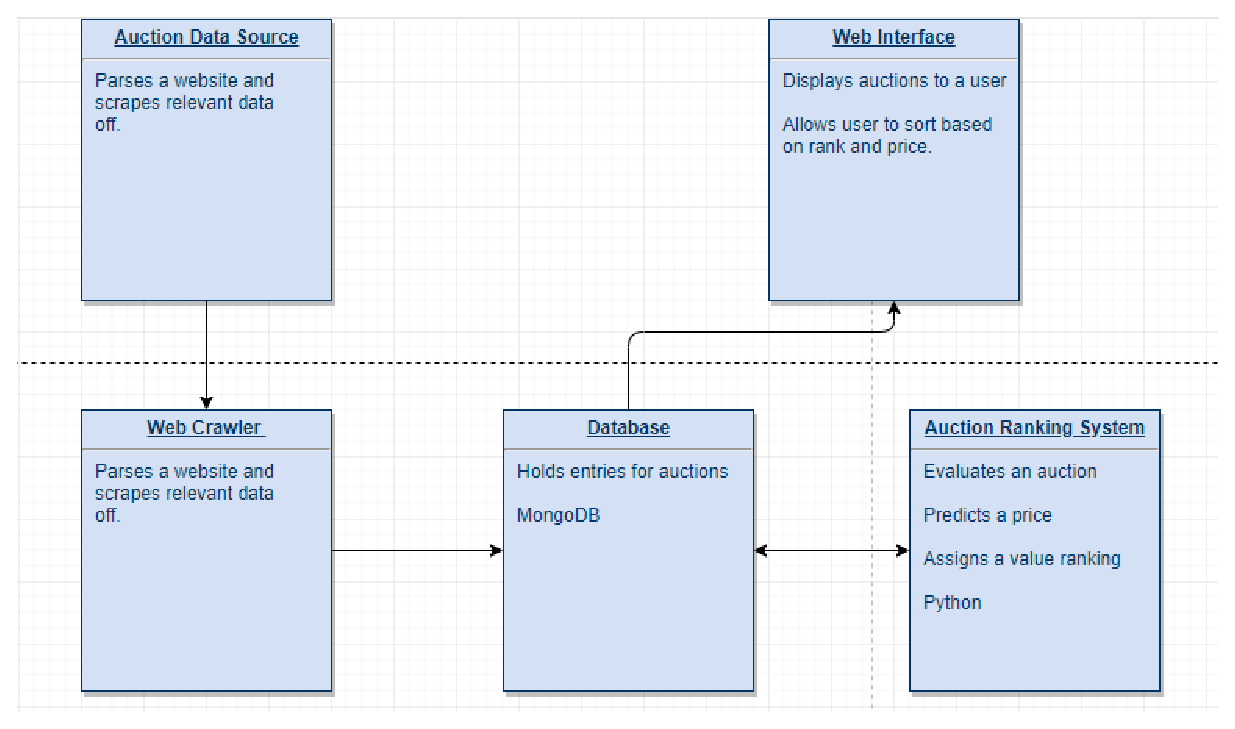
\includegraphics[scale=0.5]{flow_capture}
\caption{Flow Design}
\label{fig:flow}

\end{figure}

\end{frame}

\section{Proposed Implementation Components}

\subsection{MongoDB Database}
\begin{frame}[fragile=singleslide]{MongoDB Database Insert}
\begin{itemize}
\setlength\itemsep{2em}
\item Will need to take data from website and insert entries in database
\item Can use a uniform auction entry template
\item Relevant data will match 1:1 from website to database entry
\end{itemize}
\begin{figure}[ht]
\begin{itemize}


\begin{minted}{python}
db.inventory.insertOne(
   { item: "Tesla Model S", price: 12500, 
   tags: ["bumper damage"] }
)
\end{minted}

\end{itemize}
\caption{MongoDB 'insert' example}
\end{figure}

\end{frame}

\begin{frame}[fragile=singleslide]{MongoDB Database Find}
\begin{itemize}
    \setlength\itemsep{2em}
    \item Will need to extract entries from database. 
    \item Value calculation and website UI will need to perform this. 
    \item Below example finds all entries with a price greater than \$10,000.
    
\end{itemize}
\begin{figure}[ht]
\centering
\begin{itemize}

\begin{minted}{python}
db.collection.find( { price: { gt: 10000 } } )
\end{minted}

\end{itemize}
\caption{MongoDB 'find' example}
\end{figure}

\end{frame}

\subsection{Web Scraper}
\begin{frame}[fragile=singleslide]{Web Scraper}
\begin{itemize}
    \setlength\itemsep{2em}
    \item Web crawler will gather data from auction websites and compile in one place. 
    \item IAAI.com and Copart.com will be our primary source.
    \item Provides lots of relevant vehicle and damage information. 
    \item Scappy is a web scraper, below is how to generate one: 
\end{itemize}

\begin{figure}[ht]
\centering

\begin{minted}{python}
#create a basic spider "timedauctions"
scrapy genspider timedauctions
https://www.iaai.com/TimedAuctions
\end{minted}

\caption{Scrape Example}
\end{figure}

\end{frame}




\subsection{Auction Data Source}
\begin{frame}{Auction Data Source}

\begin{figure}[ht]
\centering
\includegraphics[scale=0.3]{timedauctions}
\caption{IAAI Timed Auctions Page}
\label{fig:auction}
\end{figure}

\end{frame}

\begin{frame}{Auction Preview Data}

From this previous page, at least the following data needs to be extracted:

\begin{itemize}
\setlength\itemsep{1em}
\item Salvage car Photos\\
\item Current bid\\
\item VIN\\
\item Time remaining\\
\item Make/Model\\
\item Damage information\\
\end{itemize}

\end{frame}

\begin{frame}[fragile=singleslide]{Extracting Info}
\textbf{Extracting the URLs include salvage car photo:}
\begin{itemize}
    \item Using developer tools of Chrome, we found photos are stored under vis.iaai.com with imageKeys:
\end{itemize}
\begin{figure}[ht]
\centering
\includegraphics[width=50mm]{salvagecarphoto}
\caption{Developer tools to find keys}
\label{fig:salvage}
\end{figure}
\begin{minted}{python}
#the attribute "imageKeys" can extract image URLs. 
response.css("img::attr(imageKeys)").extract()
\end{minted}
\end{frame}

\begin{frame}[fragile=singleslide]{Extracting Info}
\textbf{Extracting the URLs include salvage car current bid:}
We can use a similar method to find VIN's location which is attributed of the  \textless tbody\textgreater  tag.

A screen shot is available on the next page.

\begin{figure}[ht]
\begin{itemize}
\begin{minted}{python}
response.css("tbody::attr(vin)").extract()
\end{minted}
\end{itemize}
\caption{Extract Example}
\end{figure}


\end{frame}

\begin{frame}{HTML Example}

\begin{figure}[ht]
\centering
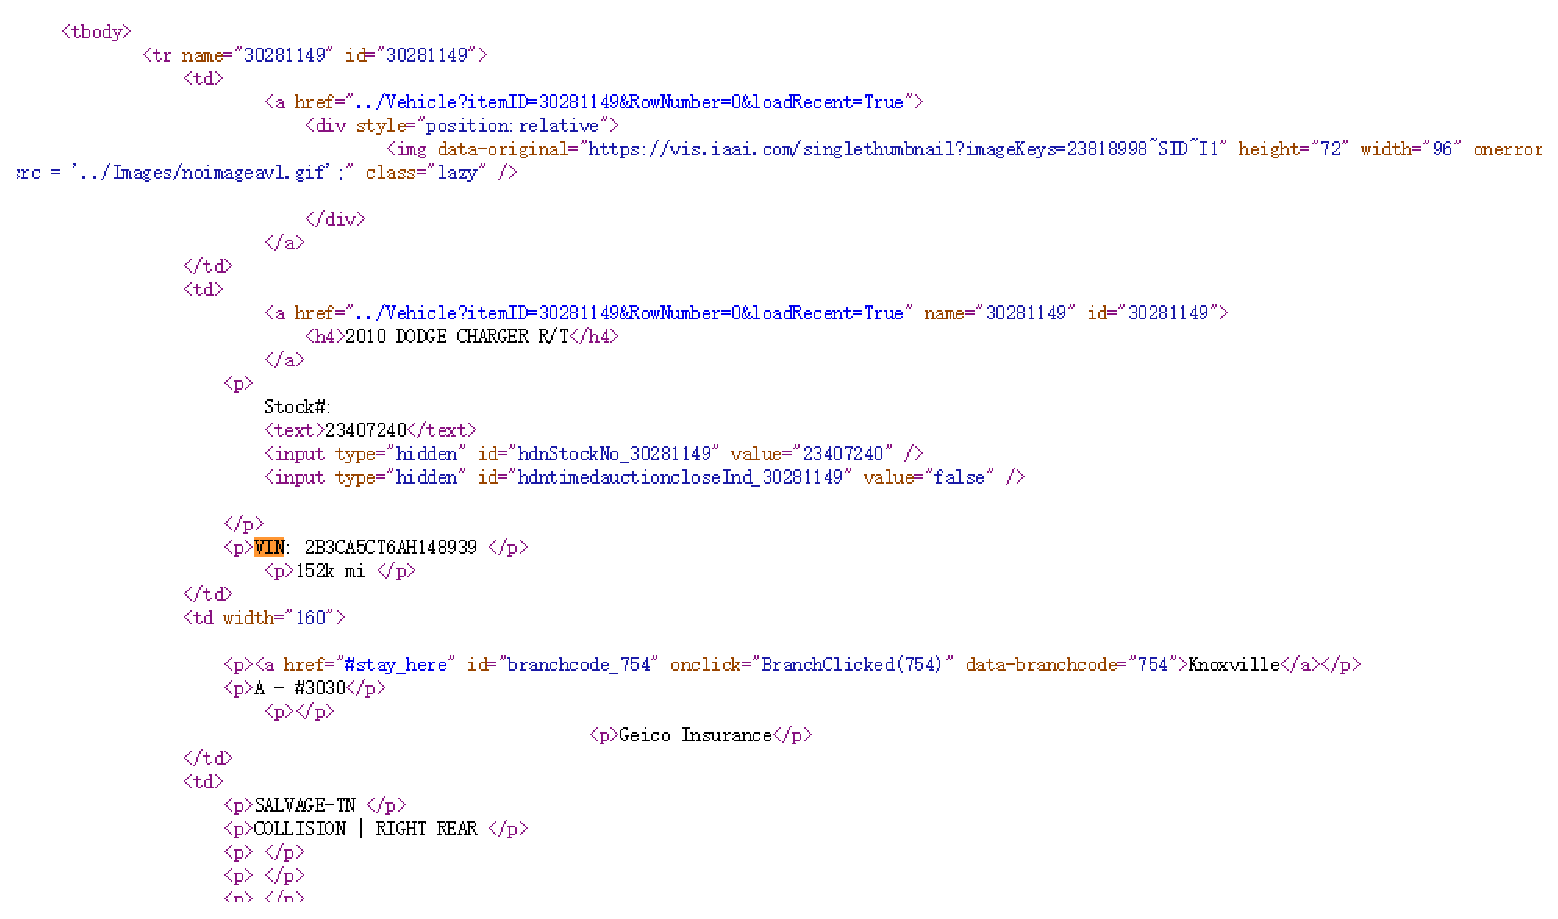
\includegraphics[width=100mm]{salvagecarvin}
\caption{Salvage Car Vin}
\label{fig:vin}
\end{figure}

\end{frame}

\begin{frame}{Extracting Info}
\textbf{Extracting the URLs include salvage car remaining time and price:}

Similarly, we are able to extract the remaining time and price of salvage car.

\textbf{Time to download the extracted photos of salvage car:}

As mentioned in Design Document, Scrapy provides the images pipelines: once we got the data from website, we are able to pass them through different pipelines. By taking advantage of this function, the image pipeline allows us to download extracted photos of salvage car. In addition, we are able to convert the format of images and generate thumbnail.
\end{frame}

\begin{frame}[fragile=singleslide]{Extracting Info}
\begin{minted}{python}
#enable the images pipeline.

SalvageCarPhotos\_PIPELINES=
'scrapy.pipelines.images.ImagesPipeline': 1

#set the local download address.

Photo\_Store =
'Users/Desktop/SalvageCarPhotos/'

#Generate two kinds of thumbnail for each salvage
car photo, one small, one large.

GenerateThumbnail = {'small': (20, 20),
'large': (100, 100)}

\end{minted}
\end{frame}

\subsection{Auction Ranking System}

\begin{frame}{Auction Ranking System}

\begin{itemize}
    \setlength\itemsep{2em}
    \item Calculates perceived value based on scraped auction data
    \item Compares posted price to perceived value to find "good deals"
    \item Will require lots of tuning and evaluation 
    \item Will use python for ease of use and compatibility with other components

\end{itemize}

\end{frame}

\subsection{Website Interface}

\begin{frame}{Website Interface}

\begin{itemize}
    \setlength\itemsep{2em}
    \item Displays sorted auctions to user
    \item Allows user to find "best deals" as evaluated by ranking system
    \item Takes useful data off source website and displays to user
    \item Allow user to automatically bid on auctions

\end{itemize}

\end{frame}

\section{Retrospective}

\begin{frame}{Weeks 1-3}
    Week 1
    \begin{itemize} % Positives
        \item Fictional Biography, Resume peer review. 
    \end{itemize}
    \hrulefill\\
    Week 2
    \begin{itemize} % Positives
        \item Selected a project and contacted client. Established mode of communication (Slack and Discord)
    \end{itemize}
    \hrulefill\\
    Week 3
    \begin{itemize} % Positives
        \item Met with client and drafted individual problem statements.
    \end{itemize}
\end{frame}


\begin{frame}{Weeks 4-6}
    Week 4
    \begin{itemize} % Positives
        \item Combined the best components from each individual problem statement for group final draft. 
    \end{itemize}
    \hrulefill\\
    Week 5
    \begin{itemize} % Positives
        \item Drafted up the majority of our requirements document. Contacted client to get initial feedback.  Started to look into available technologies for implementation.
    \end{itemize}
    \hrulefill\\
    Week 6
    \begin{itemize} % Positives
        \item Finished requirements document. Split our project into 9 categories and assigned 3 to each member for the tech review. Completed rough draft of tech review. 
    \end{itemize}
\end{frame}

\begin{frame}{Week 7-10}
    Week 7
    \begin{itemize} % Positives
        \item Applied all feedback from tech peer review. Worked on tech review final. 
    \end{itemize}
    \hrulefill\\
    Week 8
    \begin{itemize} % Positives
        \item Finished tech review final. Began gathering code snippets for implementation. 
    \end{itemize}
    \hrulefill\\
    Week 9
    \begin{itemize} % Positives
        \item Individually worked on components of the design document over the holiday weekend, then compiled our work and pieces from technology review. 
    \end{itemize}
    Week 10
    \begin{itemize} % Positives
        \item Finished design document and working on progress update, progress video, and gaining client approval. 
    \end{itemize}
\end{frame}

\end{document}